
\documentclass[10pt,a4paper]{article}

% -------------------------------------------------------------------
% packages 
% -------------------------------------------------------------------
%\usepackage{markdown}
% muss an erster stelle
\usepackage{geometry}
\usepackage{multicol}
\usepackage{amsmath,amsthm,amsfonts,amssymb}
\usepackage{graphicx,overpic}
\usepackage{color, colortbl}
\usepackage{hyperref}
\usepackage{listings}
\usepackage{mdframed}
\usepackage{minted}
\usepackage{enumitem}
%
% fuer dei pvalue tabelle
\usepackage[T1]{fontenc}
\usepackage{lmodern}
\usepackage{multicol}   % für mehrspaltiges Layout
\usepackage{booktabs}   % für schönere Tabellenlinien
\usepackage{amsmath}    % für mathematische Umgebungen
\usepackage{comment}
% -------------------------------------------------------------------
% parameters 
% -------------------------------------------------------------------

% margins & spacing 
\geometry{margin = 0.5in}
%\pagestyle{empty}
\setlength{\parindent}{0pt} 
\setlength{\parskip}{0pt}
\usepackage{xcolor}
 % box style
\begin{comment}
\lstset{ 
    numbers=left,
    basicstyle = \ttfamily,
    frame = single,
    rulecolor=\color{green},
    breaklines = true,
    columns = fullflexible,
    stringstyle=\color{DarkGreen},
    otherkeywords={0,1,2,3,4,5,6,7,8,9},
    morekeywords={TRUE,FALSE},
    deletekeywords={data,frame,length,as,character},
    keywordstyle=\color{blue},
    commentstyle=\color{DarkGreen},
}
\end{comment}

% hyperlinks 
\hypersetup{
    colorlinks = true,
    linkcolor = blue,
    filecolor = magenta,      
    urlcolor = cyan,
}


\usepackage{tcolorbox}
\usepackage[utf8]{inputenc}
\usepackage{color,soul}
\usepackage{fourier}
\usepackage{verbatim}
\setul{0.5ex}{0.3ex}
\setulcolor{red}
\renewcommand\fbox[1]{\fcolorbox{red}{white}{\textbf{ #1}}}% multicol parameters
\newcommand\fboxyellow[1]{%
    {\setlength{\fboxrule}{2pt}% Rahmenbreite nur hier ändern
    \fcolorbox{yellow}{white}{\large #1}}%
}% multicol parameters
\setlength{\fboxrule}{2pt} % Rahmenbreite auf 2pt setzen
\setlength{\premulticols}{2pt}
\setlength{\postmulticols}{2pt}
\setlength{\multicolsep}{2pt}
\setlength{\columnsep}{20pt}
% -------------------------------------------------------------------
% functions & environments 
% -------------------------------------------------------------------

% mono space font 
\newcommand{\code}[1]{\texttt{#1}}

\definecolor{codegreen}{rgb}{0,0.6,0}
\definecolor{codegray}{rgb}{0.5,0.5,0.5}
\definecolor{codepurple}{rgb}{150, 150, 150}
\definecolor{backcolour}{rgb}{230, 230, 230}
\definecolor{anti-flashwhite}{rgb}{0.95, 0.95, 0.96}
\lstdefinestyle{mystyle}{
    backgroundcolor=\color{backcolour},   
    commentstyle=\color{codegreen},
    keywordstyle=\color{black},
    numberstyle=\tiny\color{codegray},
    stringstyle=\color{codepurple},
    basicstyle=\ttfamily,
    breakatwhitespace=false,         
    breaklines=true,    captionpos=b,                    
    keepspaces=true, numbers=left,                    
    numbersep=5pt, showspaces=false,                
    showstringspaces=false, showtabs=false, tabsize=2,
    frame = single,
    rulecolor=\color{green},
    otherkeywords={0,1,2,3,4,5,6,7,8,9},}
\lstset{style=mystyle, language=R}
\newenvironment{rcode}[1]
 {\VerbatimEnvironment
  \begin{minted}[
    breaklines,
    frame=single,fontsize=\small,
bgcolor=anti-flashwhite,
    linenos]{R}}
 {\end{minted}}
% -------------------------------------------------------------------
% functions & environments 
% -------------------------------------------------------------------

\begin{document}
 \textcolor{codepurple}{meow}
\begin{multicols*}{2}
\raggedcolumns
\section{Einlesen}
\subsection{\fbox{read\_csv - read\_csv2}}
\textbf{Erzeugt Tibble}\\
\textbf{read\_csv}: Komma zum Zeilentrennen und Punkt für Dezimalzahlen\\
\textbf{read\_csv2}: Semicolon zum Zeilentrennen und Komma für Dezimalzahlen
\begin{rcode}{1]}
read_csv(file = "", col_types = "")
read_csv2(file = "", col_types = "")
\end{rcode}
Mit col\_types können wir als String wo jede Position für die jeweilige Spalten steht den Typ bestimmen\\
\textbf{Typen:}
\begin{itemize}[noitemsep]
  \item \textbf{c} = character
  \item \textbf{i} = integer
  \item \textbf{n} = number
  \item \textbf{d} = double
  \item \textbf{l} = logical
  \item \textbf{f} = factor
  \item \textbf{D} = date
  \item \textbf{T} = date time
  \item \textbf{t} = time
  \item \textbf{?} = guess
  \item \textbf{\_ oder -} = skip
\end{itemize}
\begin{rcode}{1]}
# Csv with ";" separator and "." as decimal point
read.csv("europe.data.csv", sep = ";", dec=".")

# Csv without first line as header
read.csv2("mpg.csv", header=F)

# Csv with 4 integer columns
read_csv2("magnets_pain.csv", 
            col_types = "iiii")
\end{rcode}
\subsection{\fbox{read.csv - read.csv2}}
\textbf{Erzeugt Dataframe}
\begin{rcode}{1]}
data <- read.csv(file="", sep = ";", dec = ".") %>% as_tibble()
\end{rcode}
\begin{itemize}[noitemsep]
  \item \textbf{sep} = Das Zeichen welches die Spalten trennt.
  \item \textbf{dec} = Gibt den trenner für Dezimalzahlen an
\end{itemize}
\subsection{\fbox{read\_delim - read\_delim2}}
\textbf{Erzeugt Tibble}\\
Der Rest wie bei \_
\begin{rcode}{1]}
read_delim(file = , delim = ,col_types = "")
\end{rcode}
Mit der Option \textbf{delim} können wir festlegen, mit welchem Zeichen die Zeilen getrennt werden. 
\columnbreak
\subsection{\fbox{Tidy Data}}
\textbf{Typen:}
\begin{itemize}[noitemsep]
  \item Jede Spalte muss eine Variable sein,
  \item Eine Observation ist eine Zeile,
  \item Eine Variable ist Z.b das Alter,
  \item Die einzelnen Daten sind die Beobachtungen
\end{itemize}

\normalsize
\section{\fbox{Tidying Data}}
\subsection{\fbox{pivot\_longer()}}
\textbf{Wir haben eine Tabelle wo es Spalten gibt die als Variablen selber Observationen haben. Wir wollen diese Observationen auch als Observationen hinschreiben}\\

\frame{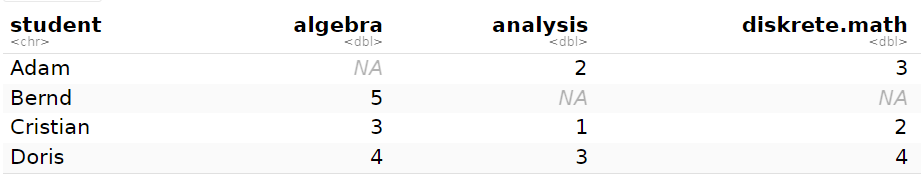
\includegraphics[draft=false, width=1\linewidth]{Figures/pivotlonger.png}}
Wir sehen, dass algebra etc eigentlich Observations sind.
\begin{rcode}{1]}
student1 %>% pivot_longer(cols =          algebra:diskrete.math, names_to = "classes", values_to = "grade", values_drop_na = T)
\end{rcode}
\begin{itemize}[noitemsep]
  \item \textbf{cols} = ein c() mit allen spalten oder spalte\_1 : spalte\_n.,
  \item \textbf{names\_to} = In welche Spalte die Namens aus cols.,
  \item \textbf{values\_to} = In Welche Spalte die Werte die in den Spalten aus cols waren,
  \item \textbf{values\_drop\_na} = T falls wir NAs droppen wollen
\end{itemize}
\frame{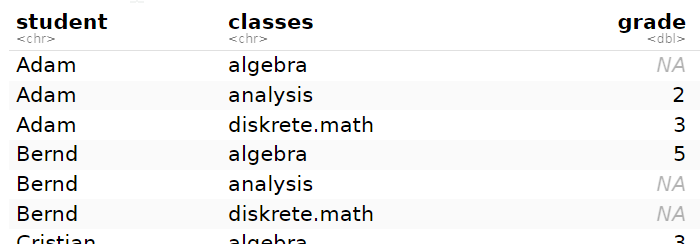
\includegraphics[draft=false, width=1\linewidth]{pivotlonger2.png}}
Hier haben wir jetzt in jeder Spalte eine Variable
\subsection{\fbox{pivot\_longer}}
Wir haben in einer Spalte für jede Observation zwei Variablen und in einer anderen Spalte die Observation für jede Variable
\frame{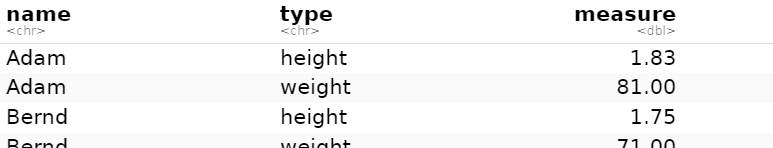
\includegraphics[draft=false, width=1\linewidth]{pivotwider.png}}
Jede Variable in Type soll eine eigene Spalte bekommen
\begin{rcode}{1]}
student2 %>% pivot_wider(names_from = type, values_from = measure)
\end{rcode}
\begin{itemize}[noitemsep]
  \item \textbf{names\_from} = Die Spalte in der die Variablen stehen.,
  \item \textbf{values\_from} = Die Spalte wo die Observationen drinne stehen.
\end{itemize}
\frame{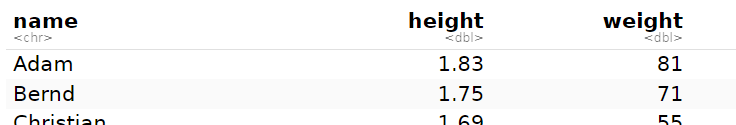
\includegraphics[draft=false, width=1\linewidth]{Figures/pivotwider2.png}}
Jetzt hat jede Variable eine Spalte
\newpage
\section{\fbox{separate}}
Wir haben in einer Spalte Zwei Observations in einer Zelle
\frame{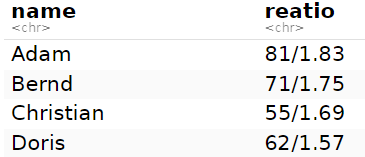
\includegraphics[draft=false, width=1\linewidth]{Figures/seperate.png}}
Nun wollen wir diese Spalte aufteilen


\begin{rcode}{1}
student3 %>% separate(col = reatio, sep = "/", into = c("weight", " height"))
\end{rcode}
\begin{itemize}[noitemsep]
  \item \textbf{col} = Die Spalte in der die Observations sind.
  \item \textbf{sep} = Das Zeichen, welches die Observations trennt.
  \item \textbf{into} = Ein Array in welches die Observations nun geschrieben werden sollen.
\end{itemize}
\frame{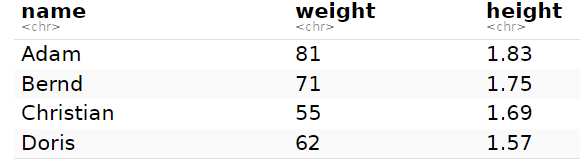
\includegraphics[draft=false, width=1\linewidth]{Figures/separate2.png}}
\begin{comment}
\begin{markdown}
# Wichtige Befehle
## Librarys
```R
library(tidyverse)
library(TeachingDemos)
```

## Datenerzeugung
- **sample** = Erzeugt ein sample aus den Werten in dem Array x mit der Länge size. Replace auf True wenn wir nur Unique werte aus x wollen.
- **runif** = Ein array mit länge n mit werten von min bis max

```R
students <- tibble(
  id = 1:10,
  sex = sample(x = c("f", "m"), size = 10, replace = T),
  age = round(runif(n = 20, min = 10, max = 35)),
)
```

\end{markdown}

\end{comment}

\end{multicols*}
\section{Probability}
\subsection{Basic Rules}

\begin{table}[h]
    \centering
    \begin{tabular}{|l|l|l|}
  \hline
        $P(A^c)$ & $1-P(A)$ & Probability that $A$ will not happen \\ 
  \hline
        $P(\emptyset)$ & $0$ & Probability of a null Event \\ 
  \hline
        $P(A \cap B)$ & \begin{tabular}{c}$P(A) * P(B)$  \\ $P(A|B)*P(B)$\end{tabular} & Probability of $A$ and $B$ occurring \\ 
  \hline
        $P(A \setminus B)$ & $P(A) - P(A \cap B)$ & Probability of $A$ without $B$ \\ 
  \hline
        $P(A \cup B)$ & $P(A) + P(B) - P(A \cap B)$ & Probability of $A$ or $B$ occurring \\ 
  \hline
        $P(A|B)$ & $\frac{P(A \cap B)}{P(B)}$ & Probability of $A$ if $B$ already happened \\ 
  \hline
\end{tabular}
    \caption{$A, B$ = Events; $P(x)$ = Probability of Event x}
    \label{tab:my_label}
\end{table}

$A \subseteq B \implies P(A) \leq P(B)$
\begin{multicols*}{2}
\subsection{Crossproduct}
$A \times B$
\begin{rcode}{1}
omega <- expand.grid(x = 1:6, y = 1:6)
\end{rcode}

\subsection{Union}
$A \cup B$
\begin{rcode}{1}
union(x = a, y = b)
\end{rcode}

\subsection{Intersection}
$A \cap B$
\begin{rcode}{1}
intersect(x = a, y = b)
\end{rcode}

\subsection{Difference}
$A \setminus B$
\begin{rcode}{1}
setdiff(x = a, y = b)
\end{rcode}

\subsection{Examples}
\begin{rcode}{1}
# Cases where first die is 1
omega %>% filter(x = 1)
# Cases where sum of dice equals 7
omega %>% filter(x + y = 7)
# Probability of dice equals 12
count(omega %>% filter(x + y = 12)) / count(omega)
\end{rcode}
\columnbreak
\subsection{Bayes formular}
\large
$$
P(A\mid B) = \frac{P(A \land B)}{P(B)}
$$
$$
P(A\land B) = P(A\mid B) \cdot P(B)
$$
\normalsize
\end{multicols*}
\begin{multicols*}{2}
\raggedcolumns
\section{probability distributions functions}

\begin{enumerate}
    \item “d” returns the height of the probability density function
    \item “p” returns the cumulative density function
    \item “q” returns the inverse cumulative density function (quantiles)
    \item “r” returns randomly generated numbers
\end{enumerate}
dgenom
\subsection{\fbox{Normalverteilung}}
\begin{rcode}{1}
pnorm(q = , mean = , sd = )
pnorm(q = 1.96, mean = 0, sd = 1)

\end{rcode}
q = Der Wert, bis zu dem wir \(P(X \le q)\) berechnen.\\
Die Ausgabe ist die Wahrscheinlichkeit, dass \(X \le q\) gilt.\\
\textbf{Beispiel:} berechnet \(P(X \le 1.96)\) für die Standardnormalverteilung.)\\
\begin{rcode}{1}
dnorm(x = , mean = , sd = )
dnorm(x = 0, mean = 0, sd = 1)
\end{rcode}
x = Der Wert, an dem die Dichte berechnet wird.\\
\textbf{Beispiel}: gibt die Dichte der Standardnormalverteilung bei \(x = 0\) zurück.)

\bigskip

\begin{rcode}{1}
qnorm(p = , mean = , sd = )
qnorm(p = 0.975, mean = 0, sd = 1)
\end{rcode}
p = Das Quantil, also der Wahrscheinlichkeitswert (zwischen 0 und 1).\\
Die Ausgabe ist der \(x\)-Wert, sodass \(P(X \le x) = p\) gilt.\\
\textbf{Beispiel:} liefert das 97,5\%-Quantil der Standardnormalverteilung.)
\begin{rcode}{1}
rnorm(n = , mean = , sd = )
rnorm(n = 10, mean = 0, sd = 1)
\end{rcode}
n = Anzahl der zu erzeugenden Zufallswerte.\\
Die Ausgabe sind \(n\) Zufallswerte aus der Normalverteilung.\\
\textbf{Beispiel:} erzeugt 10 Zufallswerte aus einer Standardnormalverteilung.)

\columnbreak
\subsection{\fbox{Binomialverteilung}}
size = number of trials (zero or more)
\\prob = probability of success on each trial.
\begin{rcode}{1}
pbinom(q = , size = , prob = )
pbinom(q = 5, size = 10, prob = 0.3)
\end{rcode}
q = Die Anzahl der Erfolge, bis zu der \(P(X \le q)\) berechnet wird.\\
Die Ausgabe ist die Wahrscheinlichkeit, dass in \(size\) Versuchen höchstens \(q\) Erfolge erzielt werden.\\
\textbf{Beispiel:} Berechnet \(P(X \le 5)\) für eine Binomialverteilung mit 10 Versuchen und einer Erfolgswahrscheinlichkeit von 0.3.)
\begin{rcode}{1}
dbinom(x = , size = , prob = )
dbinom(x = 3, size = 10, prob = 0.3)
\end{rcode}
x = Die Anzahl der Erfolge, für die die Wahrscheinlichkeit berechnet wird.\\
\textbf{Beispiel:} Gibt die Wahrscheinlichkeit zurück, genau 3 Erfolge in 10 Versuchen zu erzielen.)
\begin{rcode}{1}
qbinom(p = , size = , prob = )
qbinom(p = 0.975, size = 10, prob = 0.3)
\end{rcode}
p = Das Quantil, also der Wahrscheinlichkeitswert (zwischen 0 und 1).\\
Die Ausgabe ist die kleinste Anzahl von Erfolgen, sodass \(P(X \le x) \ge p\) gilt.\\
\textbf{Beispiel:} Liefert das 97,5\%-Quantil der Binomialverteilung.)
\begin{rcode}{1}
rbinom(n = , size = , prob = )
rbinom(n = 10, size = 10, prob = 0.3)
\end{rcode}
n = Anzahl der zu erzeugenden Zufallszahlen.\\
Die Ausgabe sind \(n\) Zufallszahlen, die jeweils die Anzahl der Erfolge in \(size\) Versuchen darstellen.\\
\textbf{Beispiel:} Erzeugt 10 Zufallszahlen aus einer Binomialverteilung mit 10 Versuchen und einer Erfolgswahrscheinlichkeit von 0.3.)
\newpage
\subsection{\fbox{Hypergeometrische Verteilung}}
n = Nummer der Erfolge\\
M = Nummer der Misserfolge\\
k = Wie viele Versuche es gibt\\
\begin{rcode}{1}
phyper(q = , m = , n = , k = )
phyper(q = 5, m = 20, n = 30, k = 10)
\end{rcode}
q = Die Anzahl der Erfolge, bis zu der \(P(X \le q)\) berechnet wird.\\
Die Ausgabe ist die Wahrscheinlichkeit, dass bei \(k\) Ziehungen aus einer Urne mit \(m\) Erfolgen und \(n\) Misserfolgen höchstens \(q\) Erfolge erzielt werden.\\
\textbf{Beispiel:} Berechnet \(P(X \le 5)\) für eine Hypergeometrische Verteilung mit \(m = 20\), \(n = 30\) und \(k = 10\).\\

\begin{rcode}{1}
dhyper(x = , m = , n = , k = )
dhyper(x = 3, m = 20, n = 30, k = 10)
\end{rcode}
x = Die Anzahl der Erfolge, für die die Wahrscheinlichkeit berechnet wird.\\
\textbf{Beispiel:} Gibt die Wahrscheinlichkeit zurück, genau 3 Erfolge bei 10 Ziehungen zu erzielen.\\

\bigskip

\begin{rcode}{1}
qhyper(p = , m = , n = , k = )
qhyper(p = 0.975, m = 20, n = 30, k = 10)
\end{rcode}
p = Das Quantil, also der Wahrscheinlichkeitswert (zwischen 0 und 1).\\
Die Ausgabe ist die kleinste Anzahl von Erfolgen, sodass \(P(X \le x) \ge p\) gilt.\\
\textbf{Beispiel:} Liefert das 97,5\%-Quantil der Hypergeometrischen Verteilung.\\

\begin{rcode}{1}
rhyper(nn = , m = , n = , k = )
rhyper(nn = 10, m = 20, n = 30, k = 10)
\end{rcode}
nn = Anzahl der zu erzeugenden Zufallszahlen.\\
Die Ausgabe sind \(nn\) Zufallszahlen, die jeweils die Anzahl der Erfolge in \(k\) Ziehungen darstellen.\\
\textbf{Beispiel:} Erzeugt 10 Zufallszahlen aus einer Hypergeometrischen Verteilung mit \(m = 20\), \(n = 30\) und \(k = 10\).


\newpage


\section{\fbox{Expected Value und Varianz}}
\subsection{\fbox{Discrete Random Variablen}}
Erwartungswert(Mean) und Varianz einer diskreten Zufallsvariablen $X$ mit Wahrscheinlichkeitsfunktion $p(x)$
\large{
\[
E[X] = \sum_{x} x \cdot\, p\cdot(x)
\]
\[
\operatorname{Var}(X) = E\left[X^2\right] - \left(E\left[X\right]\right)^2
\]
}
\normalsize
\begin{rcode}{1}
no_car <- 0.2
one_car <- 0.7
two_cars <- 0.1
expected_value <- (0*no_car) + (1*one_car) + (2*two_cars)
var <- ((0^2*no_car) + (1^2*one_car) + (2^2*two_cars)) - expected_value^2  
\end{rcode}
Hier Berechnen wir erst Mean und dann die Var. Um zur SD zu gelangen müssen wir sqrt()\\
Um jetzt herauszufinden Wieviele Parkplätze wir bauen müssen um 99\% der Autos parken zu können. Müssen wir die Anzahl der Häuser mal dem expected Value und Var rechnen
\begin{rcode}{1}
n <- 1000
qnorm(.99, mean = n*expected_value, sd=sqrt(n*var))
\end{rcode}
\subsection{\fbox{X ist Binomialy distributed}}
\large
\[
E[X] = n \cdot p \quad, \quad \operatorname{Var}(X) =n \cdot p \cdot (1-p)
\]
\subsection{\fbox{Brauche ich hier wohl uniformly und hyper?????}}
\normalsize
\columnbreak
\section{\fbox{Central Limit Theorem}}
\subsection{\fbox{Nach Maximum Sample size Umstellen $n$}}
\normalsize
\large{\textcolor{red}{\warning} Hier sollte alpha 0.5 sein, sonst 
Brute force \textcolor{red}{\warning}}\\
-\\
\normalsize
Quantilgleichung die bei der Normalapproximation der Binominalverteilung angewendet wird:
\large
\[
k + 0.5 = n \cdot p + \operatorname{qnorm}(\alpha) \cdot \sqrt{n \cdot p \cdot (1-p)}
\]
\normalsize
Wir wissen, das wenn alpha = 0.5, ist qnorm(0.5) $=0$.\\
Damit können wir $\sqrt{n \cdot p \cdot (1-p)}$ ignorieren!\\
- Jetzt haben wir also:\\
\large
\[
k + 0.5 = n \cdot p \quad\Longrightarrow\quad n = \frac{k+0.5}{p}
\]
\normalsize
\large{\textbf{Beispiel:}}
\normalsize
Aus den Fakultäten B (25\%) und C (30\%) stammen insgesamt 55\% aller Studierenden. Bei einer zufällig gezogenen Stichprobe der Größe n ist die Anzahl X der Studierenden aus B und C binomialverteilt, also X ~ Bin(n, 0,55). Ein Raum bietet 80 Plätze, weshalb die Bedingung. Der Raum soll mit eine Chance von 50\% ausreichen\\
P(X <= 80) >= 0,5
erfüllt sein muss. Bestimme das maximale n, für das diese Anforderung gilt.\\
\[
k = 80,\quad p = 0.55,\quad \alpha = 0.5,\quad \operatorname{qnorm}(0.5) = 0
\]\[
n = \frac{80.5}{0.55} \approx 146.36.
\]

\begin{rcode}{1}
n <- 80.5 / 0.55 #146.3636
\end{rcode}
Hier ist mein Bureforce Ansatz:
\begin{rcode}{1}
new_p <- b + c
new_n <- 130:150
x <- pbinom(80, new_n, new_p)
x
new_n[max(which(x >= 0.5))] #146
\end{rcode}
\section{Distributions}

\subsection*{\centering\fbox{Binominale Distribution mit zurücklegen}}
\begin{center}
\textcolor{red}{\warning}\textcolor{red}{\warning} Mit zurücklegen \textcolor{red}{\warning}\textcolor{red}{\warning}
\end{center}
\[ 
P(X = k) \;=\; \binom{n}{k}\,p^k\,(1-p)^{\,n-k} 
\]
\large{\textbf{Beispiel:}}
\normalsize
Wir haben 7 Weiße Bälle und 3 Rote Bälle:
Wie Wie groß ist die Wahrscheinlichkeit, dass wir in $n$=5 Zügen $k$=2 rote Bälle ziehen? $p$ ist 7/10

\[
P(X = 2) = \binom{5}{2} \left(\frac{3}{10}\right)^2 \left(\frac{7}{10}\right)^3.
\]
\normalsize
\begin{lstlisting}
dbinom(x = 2, size = 5, prob = 3/10)
#0.1029193
\end{lstlisting}
\[
    \begin{aligned}
    &x:\quad \text{Wie viele Rote Bälle wir bekommen wollen},\\
    &size:\quad \text{Wie Oft wir ziehen},\\
    &prob:\quad \text{Die prob einen Roten Ball zu ziehen}
    \end{aligned}
\]
%%%%%
\subsection*{\centering\fbox{Hypergemoetric Distribution ohne zurücklegen}}
\begin{center}
\textcolor{red}{\warning}\textcolor{red}{\warning} Wie Binomial, aber ohne Zurücklegen \textcolor{red}{\warning}\textcolor{red}{\warning}
\end{center}
\[
P(X = k) 
= \frac{\binom{M}{k}\,\binom{N - M}{\,n - k}}{\binom{N}{n}}
\]
\normalsize
\[
\begin{aligned}
&N:\quad \text{Gesamtanzahl aller Elemente(z.B alle Kugeln)},\\
&M:\quad \text{Anzahl der Roten Kugeln gesamt},\\
&n:\quad \text{Wie oft wir Ziehen},\\
&k:\quad \text{Wie viele Roten wir Ziehen}
\end{aligned}
\]
\begin{lstlisting}
dhyper(x = 2, m = 3,n = 7,k = 5)
#0.4166667
\end{lstlisting}
\normalsize
\[
\begin{aligned}
&x:\quad \text{wie viele von den gezogenen Bällen Rot sein sollen},\\
&M:\quad \text{wie viele Rote Bälle},\\
&n:\quad \text{wie viele nicht Rote},\\
&k:\quad \text{wie viele Bälle wir ziehen}
\end{aligned}
\]

%%%%%
\subsection*{\centering\fbox{Multinomial Distribution mit zurücklegen}}
\begin{center}
\normalsize
\textcolor{red}{\warning}\textcolor{red}{\warning} Wie Binomial aber mit mehr als zwei Optionen.\textcolor{red}{\warning}\textcolor{red}{\warning}
\end{center}

\textbf{Beispiel:}
Angenommen, wir haben $n$ = 5 Versuche.

drei mögliche Ergebnisse (z.B. rot, blau, schwarz) mit 

$Rot = \frac{15}{20},\;Grün = \frac{4}{20},\;Blau = \frac{1}{20}$.
Wir fragen: Wie groß ist die Wahrscheinlichkeit, dass genau 
$Rot$=2,\; $Grün$=2,\; $Blau$=1
\text{ auftritt?}
\[
\textbf{Formel:}\quad\frac{n!}{x_1!\,x_2!\,\cdots\,x_k!}\;p_1^{x_1}\,p_2^{x_2}\,\cdots\,p_k^{x_k},
\]
\large{\[
\frac{5!}{2!\,2!\,1!}\,\Bigl(\tfrac{15}{20}\Bigr)^2\,\Bigl(\tfrac{4}{20}\Bigr)^2\,\Bigl(\tfrac{1}{20}\Bigr)^1
= 0.3375.
\]}
\normalsize
\begin{lstlisting}
(factorial(5) / (factorial(2) * factorial(2) * factorial(1))) *
  ((15/20)^2 * (4/20)^2 * (1/20)^1)
#0.03375
\end{lstlisting}
\columnbreak
%%%%%%%
\subsection*{\centering\fbox{Multivariate Hypergeometric Distribution}}
\begin{center}
{\centering\fbox{OHNE zurücklegen}}

\normalsize
\textcolor{red}{\warning}\textcolor{red}{\warning} Wie Binomial aber mit mehr als zwei Optionen. \textcolor{red}{\warning}\textcolor{red}{\warning}
\end{center}


\textbf{Beispiel:}

Angenommen, wir haben $n$ = 5 Versuche.

drei mögliche Ergebnisse (z.B. rot, blau, schwarz) mit 

$Rot = \frac{15}{20},\;Grün = \frac{4}{20},\;Blau = \frac{1}{20}$.
Wir fragen: Wie groß ist die Wahrscheinlichkeit, dass genau 
$Rot$=2,\; $Grün$=2,\; $Blau$=1
auftritt?
\[
\textbf{Formel:}\quad
P\bigl(X_1 = k_1,\,X_2 = k_2,\,\dots,\,X_r = k_r\bigr)
= \frac{\binom{K_1}{k_1}\,\binom{K_2}{k_2}\,\dots\,\binom{K_r}{k_r}}{\binom{N}{n}}
\]
\[
\frac{\binom{15}{2}\,\binom{4}{2}\,\binom{1}{1}}{\binom{20}{5}}
\approx 0.04063467.
\]
\begin{lstlisting}
(choose(15,2) * choose(4,2) * choose(1,1)) /choose(20,5)
#0.04063467
\end{lstlisting}
%%%%%
\subsection*{\centering\fbox{Sequentielle Ziehung \textcolor{red}{mit} Zurücklegen}}
\begin{center}
\normalsize
\textcolor{red}{\warning}\textcolor{red}{\warning} mit Zurücklegen \textcolor{red}{\warning}\textcolor{red}{\warning}
\end{center}
\normalsize
\
Wir haben insgesamt 20 Bälle, davon sind 15 Bälle nicht rot
und 5 Bälle sind rot. Wir wollen die Wahrscheinlichkeit erst 4
nicht rote Bälle zu ziehen und dann ein roten Ball zu ziehen.
\begin{mdframed}[linecolor=yellow, linewidth=2pt]
P(Keinen roten Ball) = $\frac{15}{20}$

P(Einen roten Ball) = $\frac{5}{20}$
\end{mdframed}
\large{
\[\;P(X = 5)
= \Bigl(1 - \frac{15}{20}\Bigr)^{4}
\;\cdot\;\frac{4}{15}
\]}

\begin{lstlisting}
(1 - (5 / 20))^4 * 5 / 20
\end{lstlisting}


%%%%%
\subsection*{\centering\fbox{Sequentielle Ziehung \textcolor{red}{Ohne} Zurücklegen}}
\begin{center}
\normalsize
\textcolor{red}{\warning}\textcolor{red}{\warning} Ohne Zurücklegen \textcolor{red}{\warning}\textcolor{red}{\warning}
\end{center}
\normalsize
Wir haben insgesamt 20 Bälle, davon sind 15 Bälle nicht rot und 5 Bälle sind rot.
Wir wollen die Wahrscheinlichkeit erst 4 nicht rote Bälle zu ziehen und dann ein roten Ball zu ziehen.
\begin{mdframed}[linecolor=yellow, linewidth=2pt]
P(Keinen roten Ball) = $\frac{15}{20}$

P(Einen roten Ball) = $\frac{5}{20}$

P(einen roten Ball nach 4 Zügen) = $\frac{5}{16}$
\end{mdframed}

\large{
\[
P\bigl(X = 5\bigr)
= \frac{\binom{15}{4}\,\binom{5}{0}}{\binom{20}{5}} \cdot \frac{5}{16}
\]}
Wir berechnen die Wahrscheinlichkeit 4 nicht rote Bälle zu ziehen Multipliziert mit der Wahrscheinlichkeit einen roten aus den verbleibenden Bällen zu Ziehen.
\begin{lstlisting}
((choose(15,4)*choose(5,0))/choose(20,4)) * 5/16
\end{lstlisting}


\section{Type I and II Errors}
\noindent
\begin{tabular}{|l|c|c|}
\hline
& \multicolumn{2}{c|}{\textbf{True state of } $H_0$}\\
\hline
\textbf{Statistical decision} & $H_0$ True & $H_0$ False\\
\hline
\textbf{Reject $H_0$} & Type I Error & Correct\\
\hline
\textbf{Do not reject $H_0$} & Correct & Type II Error\\
\hline
\end{tabular}

\textbf{Definitions:}
\begin{itemize}
    \item $\alpha$: Probability of rejecting $H_0$ given that $H_0$ is true.
    \item $\beta$: Probability of not rejecting $H_0$ given that $H_0$ is false.
\end{itemize}

\section{Relevante Übersetzungen}
\begin{enumerate}
    \item Dispersion: Streuung (vermutlich SD gemeint)
    \item Scatter: Streuung (vermutlich SD gemeint)
\end{enumerate}
\section{P-Value}
\noindent
\noindent
\begin{tabular}{lcl}
  \toprule
  \textbf{Hypothese}         & \textbf{Test-Typ}    & \textbf{p-Wert Berechnung} \\
  \midrule
  \(H_0: \mu \ge \mu_0\)      & Einseitig (links)   & \(p = \mathtt{pnorm}(z)\)   \\
  \(H_0: \mu \le \mu_0\)      & Einseitig (rechts)  & \(p = 1 - \mathtt{pnorm}(z)\) \\
  \(H_0: \mu = \mu_0\)        & Zweiseitig          & \(p = 2 \cdot \mathtt{pnorm}(-|z|)\) \\
  \bottomrule
\end{tabular}
\section{Library}
library(TeachingDemos)
\pagebreak





















- Der Index 0 z.b. $\mu_0$ bedeutet, dass es sich um einen gegebenen Wert, und nicht um einen geschätzten Wert handelt.

\begin{center}
\fbox{I) Gauß Test:}

Hauptziel: Hier wird die Hypothese über den
Mittelwert ($\mu$) getestet
\end{center}
\begin{center}
\fboxyellow{
     {\Large{Mean \textcolor{blue}{$\mu$} ist unbekannt, wir kennen SD $\sigma$}}
}
\end{center}


\large{\textbf{Gegeben muss sein:}}
\[
H_0: \mu = \textcolor{blue}{\mu_0}, \quad H_0: \mu \leq \textcolor{blue}{\mu_0}, \quad H_0: \mu \geq \textcolor{blue}{\mu_0}
\]
\[
\begin{array}{|c|l|}
\hline
\textbf{Symbol} & \textbf{Bedeutung} \\
\hline
n & \text{Stichprobengröße} \\
\sigma_0 & \text{Standardabweichung der gesamtheit} \\
\overline{X}_{(n)} & \text{Sample Mean} \\
\hline
\end{array}
\]

\normalsize
\begin{comment}
\large{\textbf{Teststatistik:}}
\[
T = \frac{\overline{X}_{(n)} - \textcolor{blue}{\mu}}{\frac{\sigma_0}{\sqrt{n}}} \sim N(0,1)
\]
\end{comment}
\large{\textbf{Decision Rule  \(R\):}}
\[
T = \frac{\overline{X} - \textcolor{blue}{\mu_0}}{\frac{\sigma_0}{\sqrt{n}}} \in R \implies \text{reject } H_0
\]
\large{\textbf{Rejection Region \(R\):}}
\[
\begin{array}{|c|c|}
\hline
H_0 & \text{rejection region } R \\ \hline
\mu = \textcolor{blue}{\mu_0} & (-\infty, -u_{1-\frac{\alpha}{2}}) \cup (u_{1-\frac{\alpha}{2}}, \infty) \\ \hline
\mu \leq \textcolor{blue}{\mu_0} & (u_{1-\alpha}, \infty) \\ \hline
\mu \geq \textcolor{blue}{\mu_0} & (-\infty, -u_{1-\alpha}) \\ \hline
\end{array}
\]

\large{\textbf{Beispiel:}}
\begin{lstlisting}
n <- 100
sd <- 0.3
sample_mean <- 10.1
alpha <- 0.1
#H0: mu = 10, H1: mu != 10
mu0 <- 10
#Rejection region
ru <- qnorm(1-(alpha/2))
rl <- -qnorm(1-(alpha/2))
#[-1.644854, 1.644854]
#teststatistic
t <- (sample_mean - mu0) / (sd / sqrt(n))
t > ru
#3.333333
#we reject h0 because we are in the rejection region
p_value <- 1 - pnorm(t)
#0.0004290603
\end{lstlisting}
\columnbreak
\begin{center}
\fbox{II) t-Test:}
\end{center}
\normalsize
Hauptziel: Hier wird die Hypothese über den Mittelwert ($\mu$) getestet.
\begin{center}
\fboxyellow{
     \Large{Mean \textcolor{blue}{$\mu$} \ul{und} SD $\sigma_0$ sind unbekannt}
}

\textcolor{red}{\warning} Mean \textcolor{blue}{$\mu_0$} wird durch $H_0$ gegeben \textcolor{red}{\warning}
\end{center}
\large{\textbf{Gegeben muss sein:}}
\[
H_0: \mu = \textcolor{blue}{\mu_0}, \quad H_0: \mu \leq \textcolor{blue}{\mu_0}, \quad H_0: \mu \geq \textcolor{blue}{\mu_0}
\]
\[
\begin{array}{|c|l|}
\hline
\textbf{Symbol} & \textbf{Bedeutung} \\
\hline
n & \text{Stichprobengröße} \\
S_{(n)} & \text{Sample SD} \\
\overline{X}_{(n)} & \text{Sample Mean} \\
\hline
\end{array}
\]

\begin{comment}
\large{\textbf{Teststatistik:}}

\[
T = \frac{\overline{X}_{(n)} - \textcolor{blue}{\mu}}{\frac{s_{(n)}}{\sqrt{n}}} \sim t_{n-1},\text{with }
s^2_{(n)} = \frac{1}{n-1} \sum_{i=1}^n (X_i - \overline{X}_{(n)})^2
\]
\end{comment}
\large{\textbf{Decision Rule:}}
\[
T = \frac{\overline{X} - \textcolor{blue}{\mu_0}}{\frac{s_{(n)}}{\sqrt{n}}} \in R \implies \text{reject } H_0
\]

\large{\textbf{Rejection Region \(R\):}}

\[
\begin{array}{|c|c|}
\hline
H_0 & \text{Rejection Region } R \\ \hline
\mu = \textcolor{blue}{\mu_0} & (-\infty, -t_{n-1, 1-\frac{\alpha}{2}}) \cup (t_{n-1, 1-\frac{\alpha}{2}}, \infty) \\ \hline
\mu \leq \textcolor{blue}{\mu_0} & (t_{n-1, 1-\alpha}, \infty) \\ \hline
\mu \geq \textcolor{blue}{\mu_0} & (-\infty, -t_{n-1, 1-\alpha}) \\ \hline
\end{array}
\]
\large{\textbf{Beispiel:}}
\begin{lstlisting}
#H0: mu >= 250, h1: < 250
n <- 82
sample_mu <- 248
sample_sd <- 5
alpha <- 0.05
mu0 <- 250
R <- -qt(1-alpha, n-1)
#[ , -1.663884]
t <- (sample_mu - mu0) / ((sample_sd) / sqrt(n))
#-3.622154
t < r
p_value <- pt(t,n - 1)
#0.0002540167
\end{lstlisting}
\columnbreak
\begin{center}
   \fbox{III)Test für Varianz $\textcolor{blue}{\sigma_0^2}$:}
\end{center}
\normalsize

Hauptziel: Hier wird die Hypothese über die Varianz ($\textcolor{blue}{\sigma_0^2}$) getestet.
\begin{center}
\fboxyellow{
     \Large{Mean $\mu$ \ul{und} SD $\sigma$ sind unbekannt}
}

\textcolor{red}{\warning} Kein $\sigma_0$ da $\sigma$ gegeben durch $H_0$\textcolor{red}{\warning}

\textcolor{red}{\warning} Also kein Schätzwert \textcolor{red}{\warning}
\end{center}
\large{\textbf{Gegeben muss sein:}}
\[
H_0: \sigma^2 = \textcolor{blue}{\sigma_0^2}, \quad H_0: \sigma^2 \leq \textcolor{blue}{\sigma_0^2}, \quad H_0: \sigma^2 \geq \textcolor{blue}{\sigma_0^2}
\]
\[
\begin{array}{|c|l|}
\hline
\textbf{Symbol} & \textbf{Bedeutung} \\
\hline
S_{(n)}& \text{Sample SD} \\
\overline{X}_{(n)} & \text{Sample Mean} \\
\hline
\end{array}
\]
\begin{comment}
\large{\textbf{Teststatistic:}}
\[
T \;=\; \frac{(n-1)\,S_{(n)}^2}{\textcolor{blue}{\sigma^2}}
\;\;\sim\;\;\chi^2_{n-1}
\quad\text{with}\quad
S_{(n)}^2
\;=\;
\frac{1}{n-1}\sum_{i=1}^n
\bigl(X_i - \overline{X}_{(n)}\bigr)^2.
\]
\end{comment}

\large{\textbf{Decision Rule:}}
\[
T
\;=\;
\frac{(n-1)\,S_{(n)}}{\textcolor{blue}{\sigma_0^2}}
\;\in\; R
\quad\Longrightarrow\quad
\text{reject }H_0.
\]

\large{\textbf{Rejection Region \(R\):}}
\[
\begin{array}{|c|c|}
\hline
H_0 & \text{rejection region } R \\
\hline
\sigma^2 = \textcolor{blue}{\sigma_0^2}
&
(0,\;\chi^2_{n-1,\,\tfrac{\alpha}{2}})
\;\cup\;
\bigl(\chi^2_{n-1,\,1-\tfrac{\alpha}{2}},\,\infty\bigr)
\\ \hline
\sigma^2 \leq \textcolor{blue}{\sigma_0^2}
&
\bigl(\chi^2_{n-1,\,1-\alpha},\,\infty\bigr)
\\ \hline
\sigma^2 \geq \textcolor{blue}{\sigma_0^2}
&
\bigl(0,\;\chi^2_{n-1,\,\alpha}\bigr)
\\ \hline
\end{array}
\]
\large{\textbf{Beispiel:}}
\begin{rcode}{1}
#h0: sd >= 7, h1: sd <7
n <- 82
sample_mu <- 248
sample_sd <- 5
alpha <- 0.05
sd0 <- 7
#Rejection region 
R <- qchisq(alpha, n-1)
#[ , 61.26148
#Teststatistics
t <- ((n - 1) * sample_sd)/sd0
#57.85714
t < r
#We reject H0, in R area
p_value <- pchisq(t, n-1)
#0.02419782
p_value < alpha
#we reject H0
\end{rcode}
\warning Hier noch var.test 
\columnbreak
\begin{center}
   \fbox{IIII)Bernoulli Test für Probability \textcolor{blue}{$p_0$}:}
\end{center}
\normalsize

Hauptziel: Zu prüfen, ob die beobachtete Erfolgsrate $\hat{p}$ signifikant von der vorgegebenen Wahrscheinlichkeit \textcolor{blue}{$p_0$} abweicht
\begin{center}
\fboxyellow{
     \Large{Probability \textcolor{blue}{$p_0$} ist unbekannt}
}$$
\text{Number of successes: } X = \sum_{i=1}^n X_i \sim B(n, p), \quad \text{d.h. } \mathbb{E}(X) = np
$$$$
\text{Var}(X) = np(1-p).
$$
\end{center}
\large{\textbf{Gegeben muss sein:}}

\[
H_0: p = \textcolor{blue}{\textcolor{blue}{p_0}}, \quad H_0: p \leq \textcolor{blue}{p_0}, \quad H_0: p \geq \textcolor{blue}{p_0}
\]
\[
\begin{array}{|c|l|}
\hline
\textbf{Symbol} & \textbf{Bedeutung} \\
\hline
n& \text{Stichprobengröße} \\
X & \text{Number of successes} \\
\hat{p}& \frac{X}{n} \text{ Example Probability} \\
\hline
\end{array}
\]
\large{\textbf{Teststatistic}}
$$
T = \frac{\hat{p} - \textcolor{blue}{p_0}}{\sqrt{\frac{\textcolor{blue}{p_0}(1-\textcolor{blue}{p_0})}{n}}}, \quad \text{mit } \hat{p} = \frac{X}{n}.
$$
\large{\textbf{Rejection Region $R$}}
\[
\begin{array}{|c|c|}
\hline
H_0 & \text{Rejection Area } R \\ \hline
p = \textcolor{blue}{p_0} & (-\infty, -u_{1-\frac{\alpha}{2}}) \cup (u_{1-\frac{\alpha}{2}}, \infty) \\ \hline
p \leq \textcolor{blue}{p_0} & (u_{1-\alpha}, \infty) \\ \hline
p \geq \textcolor{blue}{p_0} & (-\infty, -u_{1-\alpha}) \\ \hline
\end{array}
\]
\large{\textbf{Normal Approximation:}}
\begin{rcode}{1}
#a) 80% immunity rate
#b) H0: p <= 80, H1: p > 80
p0 <- 0.8; n <- 200; x <- 172
alpha <- 0.05
phut <- x / n
#Rejection region
R <- qnorm(1 - alpha)
#r <- [0.8289439, ]
#teststatistic
t <- (phut-p0)/sqrt((p0 * (1 - p0)) / n)
#2.12132
t > R
#We reject H0
p_value <- 1 - pnorm(t)
#0.01694743
p_value < alpha
#We reject H0
\end{rcode}
\large{\textbf{Exact test:}}
\begin{rcode}{1}
#exact
binom.test(172, p = 0.8, n = n, alternative = 'greater', conf.level = 1-alpha)
#0.01793
\end{rcode}

\begin{center}
\fbox{0) Alle Infos 2-Sample Tests:}

\columnbreak
\fbox{I) 2-Sample Gauss Test:}

Hauptziel: Hier wird die Hypothese über die
Mittelwerte ($\mu_1, \mu_2$) getestet
\end{center}

\begin{center}
\fboxyellow{
     {\Large{Means  sind unbekannt, wir kennen $\sigma_1, \sigma_2$}}
}
\end{center}

\large{\textbf{Gegeben muss sein:}}
\[
H_0: \mu_1 = \mu_2, \quad 
H_0: \mu_1 \leq \mu_2, \quad 
H_0: \mu_1 \geq \mu_2
\]

\[
\begin{array}{|c|l|}
\hline
\textbf{Symbol} & \textbf{Bedeutung} \\
\hline
n_1,\,n_2 & \text{Stichprobengrößen} \\
\sigma_1,\,\sigma_2 & \text{SD der gesamtheiten} \\
\overline{X}_{(n_1)},\,\overline{Y}_{(n_2)} & \text{Sample Means} \\
\hline
\end{array}
\]

\normalsize

\large{\textbf{Teststatistik:}}
\[
T = \frac{\overline{X}_{(n_1)} - \overline{Y}_{(n_2)} - (\mu_1 - \mu_2)}
{\sqrt{\frac{\sigma_1^2}{n_1} + \frac{\sigma_2^2}{n_2}}}
\;\;\sim N(0,1)
\]

\large{\textbf{Decision Rule \(R\):}}
\[
T \in R \implies \text{reject } H_0
\]

\large{\textbf{Rejection Region \(R\):}}
\[
\begin{array}{|c|c|}
\hline
H_0 & \text{Rejection Region } R \\ \hline
\mu_1 = \mu_2 
  & (-\infty,\,-u_{1-\tfrac{\alpha}{2}})\cup(u_{1-\tfrac{\alpha}{2}},\,\infty) \\ \hline
\mu_1 \leq \mu_2 
  & (u_{1-\alpha},\,\infty) \\ \hline
\mu_1 \geq \mu_2 
  & (-\infty,\,u_{\alpha}) \\ \hline
\end{array}
\]
\large{\textbf{Beispiel:}}
\begin{lstlisting} 
m1 <-  c(5.46, 5.34, ..., 5.82)
m2 <- c(5.45, 5.31, 4.11, ..., 4.09)
sd1 <- 0.5
sd2 <- 0.6
n1 <- length(m1)
n2 <- length(m2)
#test the H0: mu1 >= mu2
alpha <- 0.05
#rejection Region
r <- qnorm(alpha)
#[ , -1.644854]
#teststistic
t <- (mean(m1) - mean(m2)) / 
  sqrt((sd1^2 / n1) + (sd2^2 / n2))
#1.027782
p_value <- pnorm(t) 
#0.8479739
#we fail to reject H0 since we are outside of the rejection area
\end{lstlisting}
\columnbreak
\normalsize
\begin{center}
\fbox{II) 2-Sample t-Test (Varianzen gleich und unbekannt):}
\normalsize
Hauptziel: Hier wird die Hypothese über die
Mittelwerte ($\mu_1, \mu_2$) getestet
\end{center}
\normalsize
\begin{center}
\fboxyellow{
     {\Large{Means $\mu_1, \mu_2$ sind unbekannt und $\sigma_1 = \sigma_2$}}
}
\end{center}

\large{\textbf{Gegeben muss sein:}}
\[
H_0: \mu_1 = \mu_2, \quad 
H_0: \mu_1 \leq \mu_2, \quad 
H_0: \mu_1 \geq \mu_2
\]
\textcolor{red}{\warning} Es muss für x und y ein Sample gegeben sein \textcolor{red}{\warning}
\large{\textbf{Beispiel:}}
\begin{comment}
\[
\begin{array}{|c|l|}
\hline
\textbf{Symbol} & \textbf{Bedeutung} \\
\hline
n_1,\,n_2 & \text{Stichprobengrößen} \\
\overline{X}_{(n_1)},\,\overline{Y}_{(n_2)} & \text{Sample Means} \\
S^2_{X,n_1},\, S^2_{Y,n_2} & \text{Sample SDs} \\
\hline
\end{array}
\]

\normalsize

\large{\textbf{Pooled Sample Variance:}}
\[
S_p^2 \;=\; 
\dfrac{(n_1 - 1)\,S_{X,n_1}^2 + (n_2 - 1)\,S_{Y,n_2}^2}
{n_1 + n_2 - 2}
\]

\large{\textbf{Teststatistik:}}
\[
T = \dfrac{\overline{X}_{(n_1)} - \overline{Y}_{(n_2)} \;-\; (\mu_1 - \mu_2)}
{S_p\,\sqrt{\dfrac{n_1 + n_2}{n_1\,n_2}}}
\;\;\sim t_{\,n_1 + n_2 - 2}
\]

\large{\textbf{Decision Rule \(R\):}}
\[
T \in R \implies \text{reject } H_0
\]

\large{\textbf{Rejection Region \(R\):}}
\[
\begin{array}{|c|c|}
\hline
H_0 & \text{Rejection Region } R \\ \hline
\mu_1 = \mu_2 
  & (-\infty,\,-t_{n_1+n_2-2,\,1-\tfrac{\alpha}{2}}) \cup (t_{n_1+n_2-2,\,1-\tfrac{\alpha}{2}},\,\infty) \\ \hline
\mu_1 \leq \mu_2 
  & (t_{n_1+n_2-2,\,1-\alpha},\,\infty) \\ \hline
\mu_1 \geq \mu_2 
  & (-\infty,\,-t_{n_1+n_2-2,\,1-\alpha}) \\ \hline
\end{array}
\]
\end{comment}
\begin{lstlisting}
x <- c(7.06, 11.84, ..., 8.54)
y <- c(8.68, 6, 7.82, 4.7, ..., 12.36)
#H0: X >= Y, H1 x < y
###################################
#case: equal variances:

t.test(x, y, alternative = 'less', paired = F, var.equal = T, conf.level = 0.95)
#p-value = 0.0181
#we can reject the h0 since we are under 0.05
\end{lstlisting}
\normalsize
\begin{center}
\fbox{III) Welsh test (Varianzen ungleich, aber unbekannt):}
\end{center}
\normalsize
Hauptziel: Hier wird die Hypothese über die
Mittelwerte ($\mu_1, \mu_2$) getestet
\normalsize
\begin{center}
\fboxyellow{
     {\Large{Means \textcolor{blue}{$\mu_1, \mu_2$} sind unbekannt und $\sigma_1 \neq \sigma_2$}}
}
\end{center}

\large{\textbf{Gegeben muss sein:}}
\[
H_0: \mu_1 = \mu_2, \quad 
H_0: \mu_1 \leq \mu_2, \quad 
H_0: \mu_1 \geq \mu_2
\]
\textcolor{red}{\warning} Es muss für x und y ein Sample gegeben sein \textcolor{red}{\warning}
\large{\textbf{Beispiel:}}
\begin{lstlisting}
x <- c(7.06, 11.84, ..., 8.54)
y <- c(8.68, 6, 7.82, 4.7, ..., 12.36)
#H0: X >= Y, H1 x < y
###################################
#case: unequal variances:
t.test(x, y, alternative = 'less', paired = F, var.equal = F, conf.level = 0.95)
#p-value = 0.01596
#we can reject the h0 since we are under 0.05
\end{lstlisting}
\fboxyellow{\textcolor{red}{\warning} Das einzige was sich ändert ist: var.equal = F\textcolor{red}{\warning}}

\columnbreak
\begin{center}
    
\fbox{IV) Two Paired Sample t-Test}
\end{center}
\textcolor{red}{\warning}Wenn Z.B einzelne Partienten vorher nacher\textcolor{red}{\warning}

\normalsize
Hauptziel: Wir berechnen als erstes den Unterschied aller Werte der beiden Samples, und dann schauen ob der Mean signifikant Unterschiedlich von 0 ist.
\normalsize
\begin{center}
\fboxyellow{
     {\Large{$\sigma$ ist unbekannt}}
}
\end{center}

\large{\textbf{Gegeben muss sein:}}
\[
H_0: \mu_1 = 0, \quad 
H_0: \mu_1 \leq 0, \quad 
H_0: \mu_1 \geq 0
\]
\textcolor{red}{\warning} Es muss für x und y ein Sample gegeben sein \textcolor{red}{\warning}
\large{\textbf{Beispiel:}}
\begin{lstlisting}
#H0: mu = 0, H1: mu != 0
x <- c(16, 15, 11, 20, ..., 15, 14, 16)
y <- c(13, 13, 10,.., 10, 15, 11, 16)
t.test(x = x, y = y, alternative = 'two.sided', paired = T, var.equal = T, conf.level = 0.95, mu = 0)
#0.0007205
\end{lstlisting}
\fboxyellow{\textcolor{red}{\warning} Das einzige was sich ändert ist: paired = T\textcolor{red}{\warning}}

\begin{center}
    
\fbox{V) Testing two Variances - F Test}
\end{center}
\normalsize
Hauptziel: Wir vergleichen die beiden sample Varianzen.
\normalsize
\begin{center}
\fboxyellow{
     {\Large{$\sigma$ ist unbekannt}}
}
\end{center}

\large{\textbf{Gegeben muss sein:}}
\[
H_0: \sigma_1 = \sigma_2, \quad 
H_0: \sigma_1 \leq \sigma_2, \quad 
H_0: \sigma_1 \geq \sigma_2
\]
\textcolor{red}{\warning} Es muss für x und y ein Sample gegeben sein \textcolor{red}{\warning}
\large{\textbf{Beispiel:}}
\begin{lstlisting}
x <- c(102.4, 101.3, ..., 100.1)
y <- c(98.4, 101.7, ..., 101.0)
#H0: sd_x <= sd_y, H1: sd_x > sd_y
alpha <- 0.05
var.test(x = x, y = y, alternative = 'greater', conf.level = 1-alpha)
#p-value = 0.03404
\end{lstlisting}

\large{\textbf{Beispiel:}}
\normalsize
Erst H0 dass vars gleich sind. Wenn nicht reject, dann müssten wir mein Mean test, var.equal auf True
\begin{lstlisting}
#H0: sigma_x = sigma_y, H1: sigma_x != sigma_y
var.test(x = x, y = y, alternative = 'two.sided', conf.level = 1-alpha)
#p-value = 0.8814
#we fail to reject H0, also Varianz gleich oder fast gleich
###############################################
#H0: mu_x <= mu_y, H1: mu_x > mu_y
alpha <- 0.025
t.test(x = x, y = y, alternative = 'greater', paired = F, var.equal = TRUE, conf.level = 1-alpha)
#p-value = 0.02374
#we reject H0
\end{lstlisting}
Wenn 

\end{multicols*}

\end{document}

% ---------------------------------------------------------------
% template 
% ---------------------------------------------------------------